%!Mode:: "TeX:UTF-8"
\documentclass[a4paper,11pt,UTF8]{ctexart}

\usepackage{indentfirst} %缩进
\usepackage{xeCJK}    %使用系统字体
\usepackage{fancyhdr} %自定义页眉页脚
\pagestyle{empty}                   %不设置页眉页脚
\usepackage{amsmath, amsthm, amssymb, amsfonts} %数学公式
\usepackage[a4paper,left=3cm,right=3cm,top=3cm,bottom=3cm]{geometry}
%\usepackage[tmargin=1in,bmargin=1in,lmargin=1.25in,rmargin=1.25in]{geometry}.
\usepackage{booktabs} %插入表格
\usepackage[section]{placeins} %避免浮动
\usepackage{listings} %插入代码
\usepackage{ctex}     %中文宏包
\usepackage[svgnames, table]{xcolor} %彩色表格
\usepackage{algorithm}          %伪代码
\usepackage{algorithmicx}
\usepackage{algpseudocode}
\usepackage{algorithm,algpseudocode,float}
\usepackage{lipsum}
\usepackage{enumitem}           %调整列举环境
\usepackage{url}
\usepackage{fontspec,xunicode}
\defaultfontfeatures{Mapping=tex-text} %如果没有它,会有一些 tex 特殊字符无法正常使用,比如连字符。

\usepackage{graphicx}
\graphicspath{{imgs/}}

%%%%%%%%%%%%%%%%%%%%%%%%%%%%%%%%%%%%%%%%%%%%%%%%%%%%%%%%%%%%%%%%
% 缩进及行间距
%%%%%%%%%%%%%%%%%%%%%%%%%%%%%%%%%%%%%%%%%%%%%%%%%%%%%%%%%%%%%%%%
\setlength{\parindent}{22pt} %重新定义缩进长度
\setlength{\baselineskip}{20pt}  %定义行间距
%\renewcommand{\baselinestretch}{1.1} %定义行间距

%%%%%%%%%%%%%%%%%%%%%%%%%%%%%%%%%%%%%%%%%%%%%%%%%%%%%%%%%%%%%%%%
% 列表设置
%%%%%%%%%%%%%%%%%%%%%%%%%%%%%%%%%%%%%%%%%%%%%%%%%%%%%%%%%%%%%%%%
\setenumerate{fullwidth,itemindent=\parindent,listparindent=\parindent,itemsep=0ex,partopsep=0pt,parsep=0ex}
\setenumerate[2]{label=\alph*),leftmargin=1.5em}  %二级item设置
\setitemize{itemindent=38pt,leftmargin=0pt,itemsep=-0.4ex,listparindent=26pt,partopsep=0pt,parsep=0.5ex,topsep=-0.25ex}
\setdescription{itemindent=38pt,leftmargin=0pt,itemsep=-0.4ex,listparindent=26pt,partopsep=0pt,parsep=0.5ex,topsep=-0.25ex}

%%%%%%%%%%%%%%%%%%%%%%%%%%%%%%%%%%%%%%%%%%%%%%%%%%%%%%%%%%%%%%%%
% 图的标题行间距设置
%%%%%%%%%%%%%%%%%%%%%%%%%%%%%%%%%%%%%%%%%%%%%%%%%%%%%%%%%%%%%%%%
\newcommand{\bottomcaption}{%
\setlength{\abovecaptionskip}{6pt}%
\setlength{\belowcaptionskip}{6pt}%
\caption}


%%%%%%%%%%%%%%%%%%%%%%%%%%%%%%%%%%%%%%%%%%%%%%%%%%%%%%%%%%%%%%%%
% 字体定义
%%%%%%%%%%%%%%%%%%%%%%%%%%%%%%%%%%%%%%%%%%%%%%%%%%%%%%%%%%%%%%%%
\setmainfont{Times New Roman}  %默认英文字体.serif是有衬线字体sans serif无衬线字体
\setmonofont{Consolas}
\setCJKmainfont[ItalicFont={楷体}, BoldFont={黑体}]{宋体}%衬线字体 缺省中文字体为
\setCJKsansfont{黑体}
\punctstyle{hangmobanjiao}
%-----------------------xeCJK下设置中文字体------------------------------%
\setCJKfamilyfont{song}{SimSun}                             %宋体 song
\newcommand{\song}{\CJKfamily{song}}
\setCJKfamilyfont{fs}{FangSong}                      %仿宋  fs
\newcommand{\fs}{\CJKfamily{fs}}
\setCJKfamilyfont{ktgb}{KaiTi}                      %楷体2312 ktgb
\newcommand{\ktgb}{\CJKfamily{ktgb}}
\setCJKfamilyfont{yh}{Microsoft YaHei}                    %微软雅黑 yh
\newcommand{\yh}{\CJKfamily{yh}}
\setCJKfamilyfont{hei}{SimHei}                              %黑体  hei
\newcommand{\hei}{\CJKfamily{hei}}
\setCJKfamilyfont{hwxk}{STXingkai}                                %华文行楷  hwxk
\newcommand{\hwxk}{\CJKfamily{hwxk}}
%------------------------------设置字体大小------------------------%
\newcommand{\shiyanbaogao}{\fontsize{36pt}{\baselineskip}\selectfont}
\newcommand{\chuhao}{\fontsize{42pt}{\baselineskip}\selectfont}     %初号
\newcommand{\xiaochuhao}{\fontsize{36pt}{\baselineskip}\selectfont} %小初号
\newcommand{\yihao}{\fontsize{28pt}{\baselineskip}\selectfont}      %一号
\newcommand{\erhao}{\fontsize{21pt}{\baselineskip}\selectfont}      %二号
\newcommand{\xiaoerhao}{\fontsize{18pt}{\baselineskip}\selectfont}  %小二号
\newcommand{\sanhao}{\fontsize{15.75pt}{\baselineskip}\selectfont}  %三号
\newcommand{\sihao}{\fontsize{14pt}{\baselineskip}\selectfont}       %四号
\newcommand{\xiaosihao}{\fontsize{12pt}{\baselineskip}\selectfont}  %小四号
\newcommand{\wuhao}{\fontsize{10.5pt}{\baselineskip}\selectfont}    %五号
\newcommand{\xiaowuhao}{\fontsize{9pt}{\baselineskip}\selectfont}   %小五号
\newcommand{\liuhao}{\fontsize{7.875pt}{\baselineskip}\selectfont}  %六号
\newcommand{\qihao}{\fontsize{5.25pt}{\baselineskip}\selectfont}    %七号

%%%%%%%%%%%%%%%%%%%%%%%%%%%%%%%%%%%%%%%%%%%%%%%%%%%%%%%%%%%%%%%%
% 图题字体大小相同
%%%%%%%%%%%%%%%%%%%%%%%%%%%%%%%%%%%%%%%%%%%%%%%%%%%%%%%%%%%%%%%%
\usepackage{caption}
\captionsetup{font={footnotesize}}   % footnotesize = 9pt
\captionsetup[lstlisting]{font={footnotesize}}

%%%%%%%%%%%%%%%%%%%%%%%%%%%%%%%%%%%%%%%%%%%%%%%%%%%%%%%%%%%%%%%%
% 重定义枚举编号为 1),2)...
%%%%%%%%%%%%%%%%%%%%%%%%%%%%%%%%%%%%%%%%%%%%%%%%%%%%%%%%%%%%%%%%
\renewcommand{\labelenumi}{\theenumi)}


%%%%%%%%%%%%%%%%%%%%%%%%%%%%%%%%%%%%%%%%%%%%%%%%%%%%%%%%%%%%%%%%
% 重定义section标题
%%%%%%%%%%%%%%%%%%%%%%%%%%%%%%%%%%%%%%%%%%%%%%%%%%%%%%%%%%%%%%%%
\CTEXsetup[format={\sihao\CJKfamily{zhhei}\zihao{4}},number={\chinese{section}},name={,、~},aftername={},indent={0pt},beforeskip={6pt},afterskip={6pt},format+={\flushleft}]{section}
\CTEXsetup[format={\Large\bfseries\CJKfamily{zhkai}\zihao{5}},name={(,)},number={\chinese{subsection}},aftername={},indent={22pt},beforeskip={14pt},afterskip={2pt}]{subsection}
\CTEXsetup[number={\chinese{section}},name={附录, ~~ }]{appendix}



%%%%%%%%%%%%%%%%%%%%%%%%%%%%%%%%%%%%%%%%%%%%%%%%%%%%%%%%%%%%%%%%
% 标题名称中文化
%%%%%%%%%%%%%%%%%%%%%%%%%%%%%%%%%%%%%%%%%%%%%%%%%%%%%%%%%%%%%%%%
\renewcommand\figurename{\hei 图}
\renewcommand\tablename{\hei 表}
\renewcommand\lstlistingname{\hei 代码}
\renewcommand{\algorithmicrequire}{\textbf{输入:}}
\renewcommand{\algorithmicensure}{\textbf{输出:}}
\newtheorem{define}{定义}

%%%%%%%%%%%%%%%%%%%%%%%%%%%%%%%%%%%%%%%%%%%%%%%%%%%%%%%%%%%%%%%%
% 代码设置
%%%%%%%%%%%%%%%%%%%%%%%%%%%%%%%%%%%%%%%%%%%%%%%%%%%%%%%%%%%%%%%%
\lstset{
 columns=fixed,
 numbers=left,                                        % 在左侧显示行号
 numberstyle=\tiny\color{gray},                       % 设定行号格式
 frame=single,                                        % 单线背景边框
 breaklines=true,                                     % 设定LaTeX对过长的代码行进行自动换行
 keywordstyle=\color[RGB]{40,40,255},                 % 设定关键字颜色
 numberstyle=\footnotesize\color{darkgray},
 commentstyle=\it\color[RGB]{0,96,96},                % 设置代码注释的格式
 stringstyle=\rmfamily\slshape\color[RGB]{128,0,0},   % 设置字符串格式
 showstringspaces=false,                              % 不显示字符串中的空格
 language=java,                                        % 设置语言
 basicstyle=\linespread{1.0}\xiaowuhao\ttfamily,                      % 字体字号
 %lineskip=10pt,
 %baselinestretch=1,
}

%%%%%%%%%%%%%%%%%%%%%%%%%%%%%%%%%%%%%%%%%%%%%%%%%%%%%%%%%%%%%%%%
% 伪代码分页
%%%%%%%%%%%%%%%%%%%%%%%%%%%%%%%%%%%%%%%%%%%%%%%%%%%%%%%%%%%%%%%%
\makeatletter
\renewcommand{\ALG@name}{算法}
\newenvironment{breakablealgorithm}
  {% \begin{breakablealgorithm}
   \begin{center}
     \refstepcounter{algorithm}% New algorithm
     \hrule height.8pt depth0pt \kern2pt% \@fs@pre for \@fs@ruled
     \renewcommand{\caption}[2][\relax]{% Make a new \caption
       {\raggedright\textbf{\ALG@name~\thealgorithm} ##2\par}%
       \ifx\relax##1\relax % #1 is \relax
         \addcontentsline{loa}{algorithm}{\protect\numberline{\thealgorithm}##2}%
       \else % #1 is not \relax
         \addcontentsline{loa}{algorithm}{\protect\numberline{\thealgorithm}##1}%
       \fi
       \kern2pt\hrule\kern2pt
     }
  }{% \end{breakablealgorithm}
     \kern2pt\hrule\relax% \@fs@post for \@fs@ruled
   \end{center}
  }
\makeatother



\begin{document}
\xiaosihao\song

\begin{titlepage}
  \center{\yihao{\ktgb{中山大学数据科学与计算机学院\\操作系统实验课程}}}
  \vspace{1cm}

  
  \center{\shiyanbaogao{\ktgb{实~验~报~告}}}
  \vspace{2cm}
  
  \begin{center}
  \begin{large}
  \begin{tabular}{rc}
  \xiaoerhao{\hei{教\qquad 师}}& \sanhao{\hei{凌应标}}\\
  \cline{2-2}\\
  \xiaoerhao{\hei{学\qquad 号}}& \hspace{1.7cm}\sanhao{\hei{17341038\hspace{1.7cm}}} \\
  \cline{2-2}\\
  \xiaoerhao{\hei{姓\qquad 名}}& \sanhao{\hei{傅畅}}\\
  \cline{2-2}\\
  \xiaoerhao{\hei{实验名称}}& \sanhao{\hei{实验三(开发独立内核的操作系统)}}\\
  \cline{2-2}\\
  
  \end{tabular}
  \end{large}
  \end{center}
  \vfill \hfill
  \end{titlepage}
  \clearpage
\clearpage

\setlength{\parskip}{6pt}  %定义段间距

\section{实验目的:用C和汇编实现操作系统内核}
  \subsection{用C和汇编实现操作系统内核}
  \subsection{增加批处理能力}
    \subsubsection{提供用户返回内核的一种解决方案}
    \subsubsection{一条在内核的C模块中实现}
      \begin{itemize}
          \item 在磁盘上建立一个表,记录用户程序的存储安排
          \item 可以在控制台查到用户程序的信息,如程序名、字节数、在磁盘映像文件中的位置等
          \item 设计一种命令,命令中可加载多个用户程序,依次执行,并能在控制台发出命令
          \item 在引导系统前,将一组命令存放在磁盘映像中,系统可以解释执行
      \end{itemize}
        

\section{实验原理:}
      \subsection{c函数与nasm函数的相互调用}
        c语言在实现比较复杂的程序逻辑上比较简单,而asm在实现底层IO功能上比较直接,本次实验的许多个功能我需要两者尽可能多地需要两者相互调用,汲取各自长处
        c语言函数的调用,在汇编中的实现方法,只是将参数简单压入栈,然后将返回出口压入栈后,直接跳向函数入口。
        知道这一点之后,汇编代码想要直接调用c函数,只需要将参数压入栈即可;asm代码段想要使用c函数传过来的参数,也只需要从$sp+4$之后的位置取出即可。
        在函数返回值在汇编层面也只是用eax来传递
      \subsection{c语言与nasm交叉编译}
        由于现阶段暂时还只能编译16bin文件,gcc的参数需要指明-m32,同时需要关闭对关联库和builtin函数。
      \subsection{obj文件的链接}
        ld对.o文件先后顺序敏感,被依赖的文件需要放在后面;而且编译出来在bin文件中相对顺序也和命令中文件顺序有关
      \subsection{执行用户程序前后的寄存器保护措施}
        所有在用户程序中被使用的寄存器,都需要使用栈加以保存。待到模块结束ret后需要弹出恢复。


\section{代码分析:}
\lstset{language=={[x86nasm]Assembler}}
	\begin{lstlisting}[caption={asm code },tabsize=4,basicstyle=\footnotesize,captionpos=b]
  \end{lstlisting}
  
\begin{lstlisting}[caption={一段C代码},captionpos=b]
  #include <stdio.h>
  int main (int argc, char *argv[]){
    printf("Hello world!");
  }
\end{lstlisting}
      \subsection{shell代码逻辑}
      \begin{lstlisting}[caption={一段C代码},captionpos=b]
void shell(){
    for (;;){
      char p[15]= "fuchang@1038 $\0";
      int len =strnlen(p, MAXLEN),i;
      puts(p, len, &row,&col);
      len=0;
      for (char ch=getchar(); ch!= '\r' && ch!='\n'; ch=getchar()){
        if ( ch==0x8 ){
          if ( len){
            --col;
            putchar(' ', &row,&col), s[--len] = 0;
            --col;setCursor(row, col);
          }
        }else{
          putchar(ch, &row,&col);s[len++] = ch;
        }
      }
      Enterline(&row, &col);
      for (i=0; s[i]==' ' && i<len;++i);
      if (i<len)exec_single(s+i, len-i);
    }
  }
      \end{lstlisting}
      整个shell的逻辑比较简单,不断输入字符并在屏幕上追踪显示;如果输入了删除符0x8则退格显示。\\
      等到输入回车换行符之后,光标换行Enterline(),并扫描命令行,跳进命令解释函数exec\_single()

      \subsection{ls现实当前文件信息}
      \begin{lstlisting}[caption={一段C代码},captionpos=b]
void dir(int showall){
	char *p;
	for (volatile int i=0; i<32; ++i){
		p=readItem(i);
		if (p[0]==0) break;
		volatile int len = p[7]=='\0'?strnlen(p,8):8,num=0;
		if ( !showall){
			if ( i) {putchar(' ', &row,&col);}
			puts(p, len, &row, &col);
		}else{
			puts(p,len, &row, &col);
			puts(" section:",9, &row, &col);putnum(sectionLoc(p), &row,&col);
			puts(" size:",6,&row, &col); putnum(fileSiz(p)<<9, &row, &col);
			num=createTim(p);
			puts(" crtime:",8, &row, &col);
			putnum(num/60,&row,&col);putchar(':',&row,&col);putnum(num%60, &row,&col);
			puts(" filetype:",10,&row, &col);
			num=fileTyp(p);
			if ( num==1) puts("bin",3, &row, &col);	else
			if ( num==2) puts("bat",3, &row, &col);	else
			if ( num==0) puts("ker",3, &row, &col);
			
			Enterline(&row, &col);
		}
	}
	if ( !showall)Enterline(&row,&col);
}
      \end{lstlisting}
      
      该ls命令会将表中的所有文件的文件名都输出\\
      另外我设计的ls命令带有一个可选参数$-al$,该参数下ls会将文件的所有详情信息全部输出。\\
      为了方便读取文件信息,我对每一条文件信息都写了对应的函数
      \begin{lstlisting}[caption={一段C代码},captionpos=b]

typedef char* itemPtr;
int sectionLoc(itemPtr p){return (((int)p[9])<<8) + p[8];}
int fileSiz(itemPtr p){ return (((int)p[11])<<8)+p[10];}
int createTim(itemPtr p){return ((  (int)p[13])<<8)+p[12];}
int fileTyp(itemPtr p){return (((int)p[15])<<8)+p[14];}
      \end{lstlisting}
      \subsection{对批处理文件与bin文件的执行}
  
      \begin{lstlisting}[caption={一段C代码},captionpos=b]
void exec_single(char *cmd, int len){
  if ( strncmp(cmd, "./",2)==0){
    int i=2,j,k;
    for (; i<len && cmd[i]==' ';++i);
    for (j=i; cmd[j]!=' ' && j<len; ++j);
    int exist=0;
    itemPtr t=readItem(k);
    for (k=0; k<32; ++k,t+=16) if ( strncmp(cmd+i,t, j-i)==0){ // bug ,t+=16?
      if ( fileTyp(t) ==1)run_user_prog(k);else
      if ( fileTyp(t) ==2)exec_batch(get_user_bat(k),fileSiz(t)<<9);
      exist = 1;
    }
    if ( !exist) puts("file not found!",15, &row,&col);
    
  }	else
  if ( strncmp(cmd, "ls",2)==0){
    int i=2, j;
    for (; i<len && cmd[i]==' '; ++i);
    for (j=i; cmd[j]!=' '&& j<len; ++j);
    if ( j-i>0){
      if (j-i==3  && strncmp(cmd+i, "-al",3)==0)
        dir(1);
      else puts("paramenter not found!",21, &row, &col);
    }else dir(0);
  }	else
    puts("command not found!",18, &row, &col);
}
      \end{lstlisting}
      该函数的解释过程其实就是对两个指令字符串的匹配过程。整个过程比较冗余的还是对非法输入的判断。\\
      对用户bin文件的执行和用户batch文件的执行还是有不同的,用户batch文件本质上还是一堆指令字符串\\
      \lstset{language=={[x86nasm]Assembler}}
  \begin{lstlisting}[caption={asm code },tabsize=4,basicstyle=\footnotesize,captionpos=b]
    bat.sh_start:
    db "./prog2",0xa,"./prog1",0xa
    times 512-($-bat.sh_start) db 0
      
  \end{lstlisting}
  
  调用nasm中的用户程序,需要加载其到对应的内存并跳转执行,这里的run\_user\_prog和get\_user\_bat用nasm写的
  都是得到目的地地址或者命令地址然后直接执行
      \lstset{language=={[x86nasm]Assembler}}
      \begin{lstlisting}[caption={asm code },tabsize=4,basicstyle=\footnotesize,captionpos=b]
run_user_prog:			;debug
        ; run user's bin prog
    push ax
    push bx

    mov bx, sp
    push word [bx+0x8]
    call dword Load_prog	
    xor ebx, ebx
    mov bx, ax
    call dword ebx

    add sp, 0x2  		;bug , fail to match the push--pop bracket 
    pop bx
    pop ax

o32 ret   

get_user_bat:
						;run user's bat order

		push bx			;each take 2 units of stack memo

		mov bx, sp
		push word [bx+0x6]
		call dword Load_prog
		add sp,0x2

		pop bx

o32	ret

      \end{lstlisting}
       
      \subsection{IO函数设计}
      我主要在nasm中封装了4个函数:
        \subsubsection{putchar}
        调用10号中断,将字符串输出到第0页的指定位置
        \lstset{language=={[x86nasm]Assembler}}
        \begin{lstlisting}[caption={asm code },tabsize=4,basicstyle=\footnotesize,captionpos=b]
asm_putchar:			;debugged
push ax
push bx
push cx
push dx
push ds
push es
push bp   ; bug, every register used in the prog must be protected !!!

  mov  ax, cs           ; 置其他段寄存器值与CS相同
  mov  ds, ax           ; 数据段
  mov  bp, sp      ; BP=当前串的偏移地址
  add bp, 0x12
  mov  ax, ds           ; ES:BP = 串地址
  mov  es, ax           ; 置ES=DS
  mov  cx,1 ; CX=串长
  mov  ax, 1301h        ; AH = 13h(功能号)、AL = 01h(光标置于串尾)
  mov  bx, 0007h        ; 页号为0(BH = 0) 黑底白字(BL = 07h)
  mov  dh, [bp+0x4]            ; 行号=0
  mov  dl, [bp+0x8]            ; bug , each is 64bit !!!
  int  10h              ; BIOS的10h功能:显示一行字符

pop bp
pop es
pop ds
pop dx
pop cx
pop bx
pop ax
o32	ret          
        \end{lstlisting}              
        \subsubsection{getchar}
        getchar实现比较简单,调用16h中断后,所得ascii码直接存在了al中,作为返回值可以直接ret
        \lstset{language=={[x86nasm]Assembler}}
        \begin{lstlisting}[caption={asm code },tabsize=4,basicstyle=\footnotesize,captionpos=b]
getchar:			;debugged
  mov ax,0x0
  int 16h
o32 ret
        \end{lstlisting}
        
        \subsubsection{屏幕下滚}
        \lstset{language=={[x86nasm]Assembler}}
  \begin{lstlisting}[caption={asm code },tabsize=4,basicstyle=\footnotesize,captionpos=b]
ScrollDown:			;debugged

    push ax
    push bx
    push cx
    push dx
  
    mov    ah,6    ;6=屏幕初始化或上卷 , 7=屏幕初始化或下卷
    mov    al,1;   AL = 上卷行数AL =0全屏幕为空白 
    mov    bh,0;   BH = 卷入行属性
    mov    cx,0; CH = 左上角行号 CL = 左上角列号 
    mov    dx,0x184f    ;DH = 右下角行号 DL = 右下角列号(24,79)
    int 10h
  
    pop dx
    pop cx
    pop bx
    pop ax
  o32 ret
      
  \end{lstlisting}
  
        \subsubsection{设置光标}
        \lstset{language=={[x86nasm]Assembler}}
  \begin{lstlisting}[caption={asm code },tabsize=4,basicstyle=\footnotesize,captionpos=b]
  setCursor: ; debugged
    push dx
    push bx
    push bp
    push ax
  
    xor ax, ax
    xor bx, bx
    mov ah, 2h
    mov bp,sp
    mov dh, [bp+0xc]  ; mad to calc the real site in stack
    mov dl, [bp+0x10]
    int 10h
  
    pop ax
    pop bp
    pop bx
    pop dx
  o32 ret
  \end{lstlisting}
  
      然后在c语言中就可以比较方便地实现puts,putnum,Enterline等函数:
      \begin{lstlisting}[caption={一段C代码},captionpos=b]
void putchar(char ch, int *r, int *c){  // used for
  asm_putchar(ch, *r, *c);
  ++(*c);
}

void puts(char *s, int len, int *r, int *c){
  for (volatile int i=0; i<len && s[i]; ++i,++(*c))
    asm_putchar(s[i], *r,*c);
} // print a string at the (r,c), used for terminal 

extern void Enterline(int *r, int *c){
  for (;(*r)>=24; --(*r))ScrollDown();
  ++(*r);*c=0;
}
void putnum(int num,int *r, int *c){
  tmplen=0;
  if ( num==0) putchar('0', r, c);	else{
    for (; num ;num/=10) tmp[tmplen++] = num%10;
    for (volatile int i=tmplen-1; ~i; --i)
      putchar(tmp[i]+'0',r, c);
  }
}
      \end{lstlisting}
      \subsection{makefile}

\section{实验结果与分析(含重要数据结果分析或核心代码流程分析):}

\begin{figure}[!htbp]
  \centering
  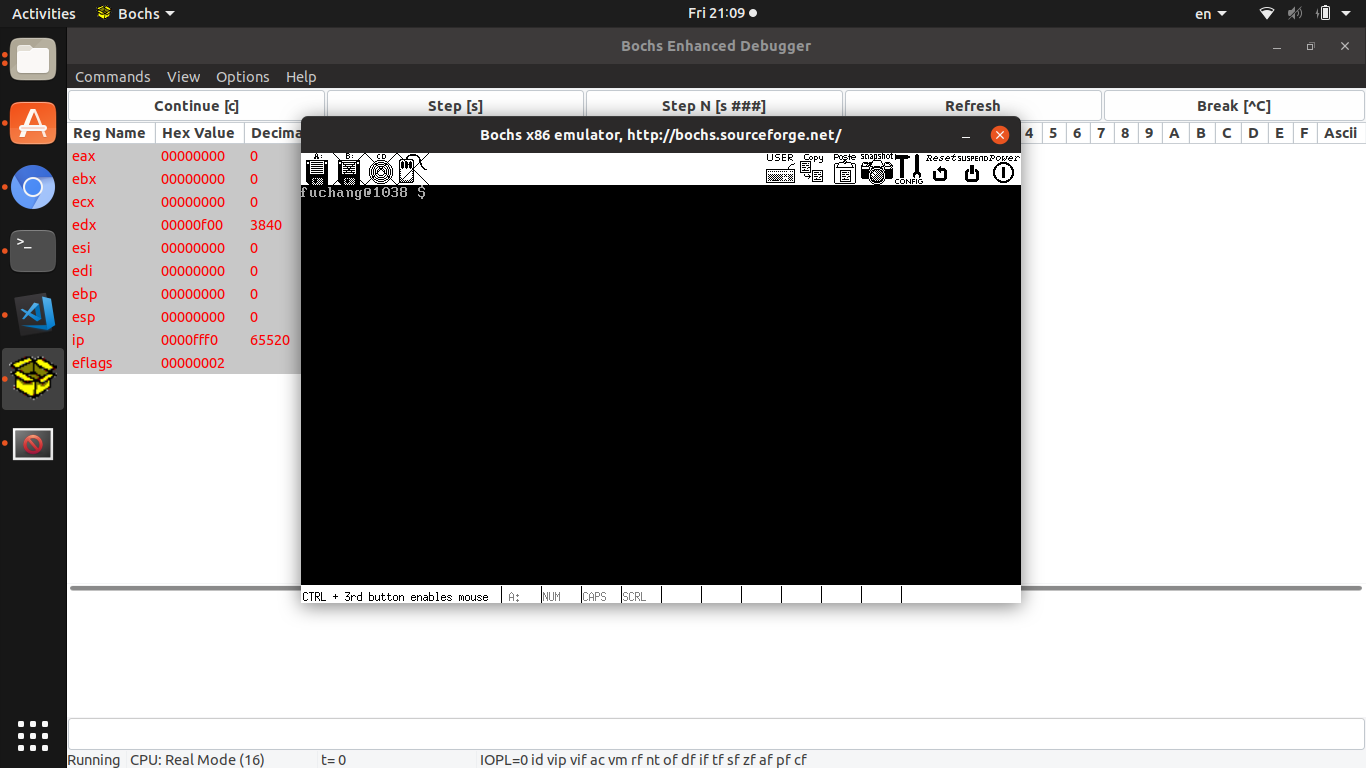
\includegraphics[width=\textwidth]{imgs/Screenshot_from_2019-03-29_21-09-42.png}
  \bottomcaption{\xiaowuhao{打开程序显示命令行}}
  \end{figure}
  
  \begin{figure}[!htbp]
  \centering
  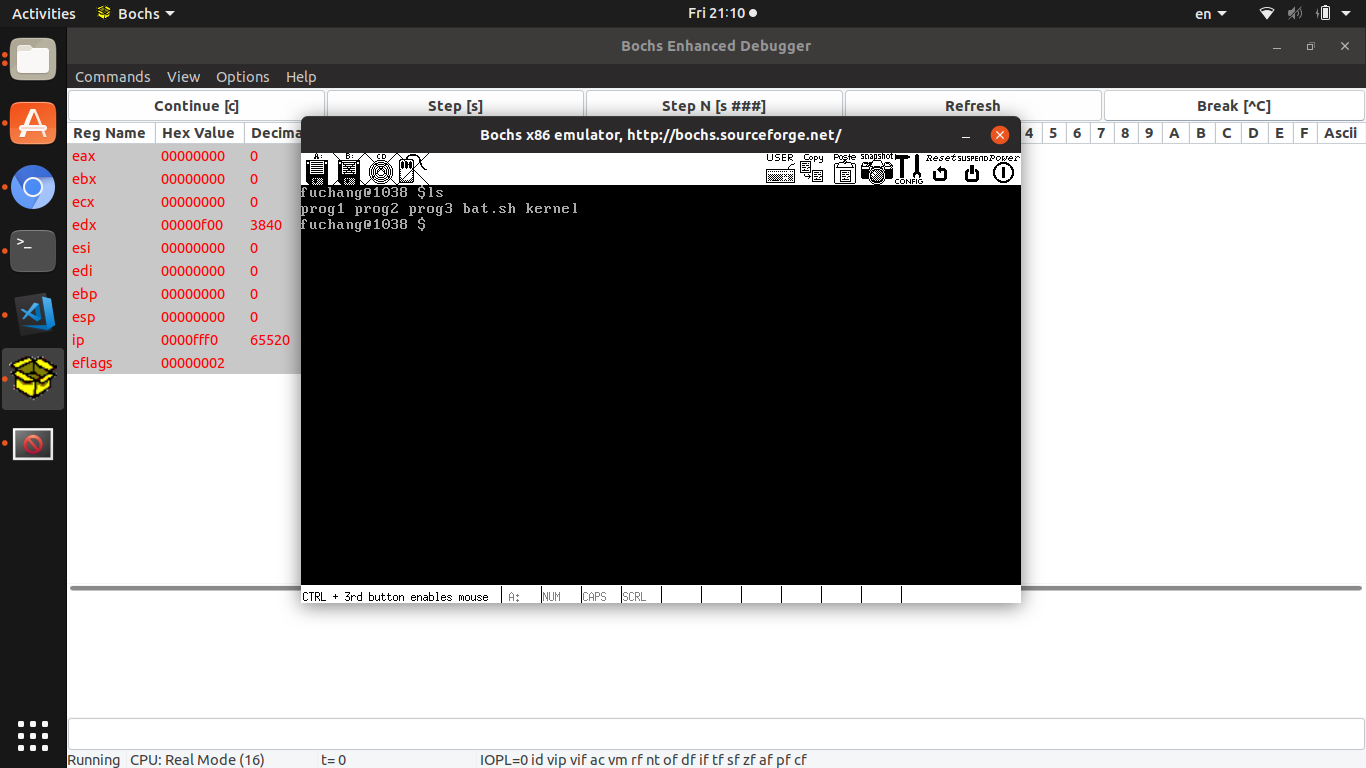
\includegraphics[width=\textwidth]{imgs/Screenshot_from_2019-03-29_21-10-06.png}
  \bottomcaption{\xiaowuhao{输入\textbf{ls}指令}}
  \end{figure}
  
  \begin{figure}[!htbp]
    \centering
    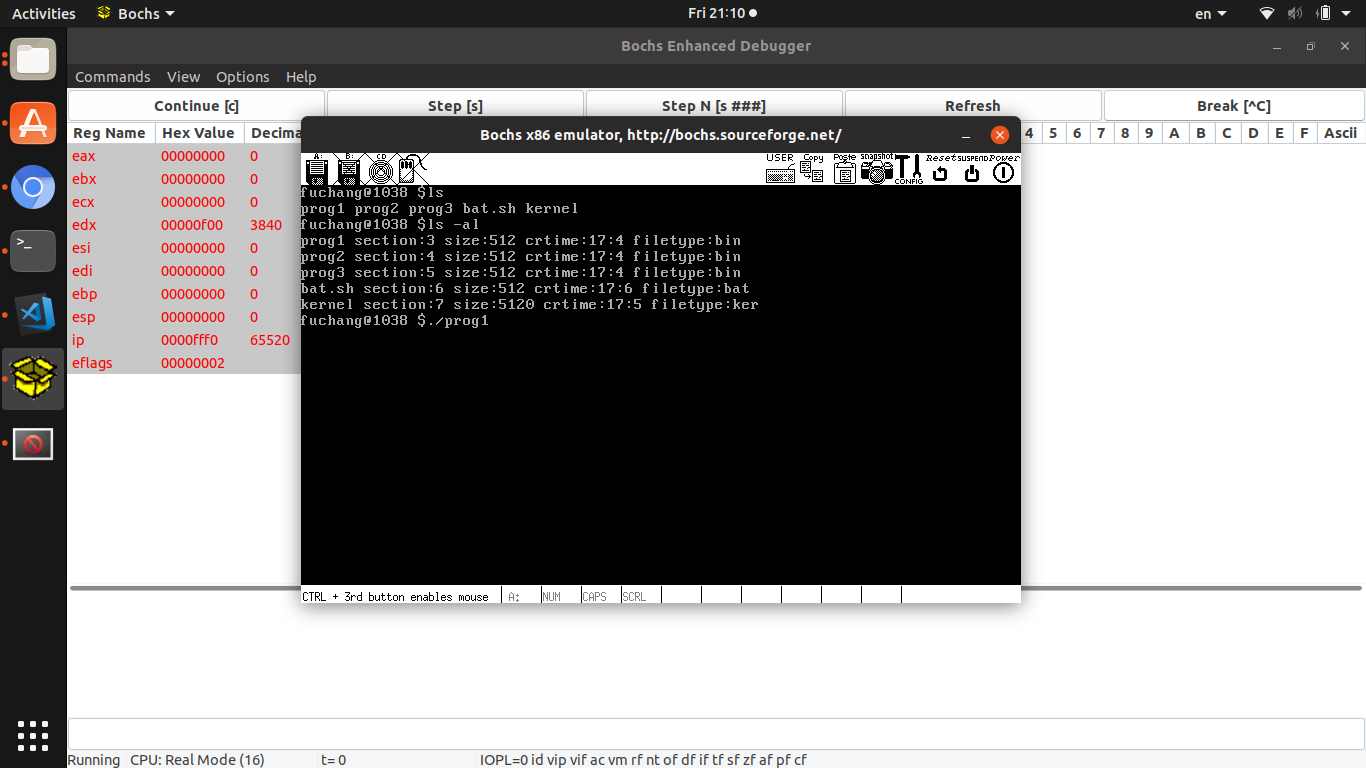
\includegraphics[width=\textwidth]{imgs/Screenshot_from_2019-03-29_21-10-28.png}
    \bottomcaption{\xiaowuhao{Shot3}}
  \end{figure}
  \begin{figure}[!htbp]
    \centering
    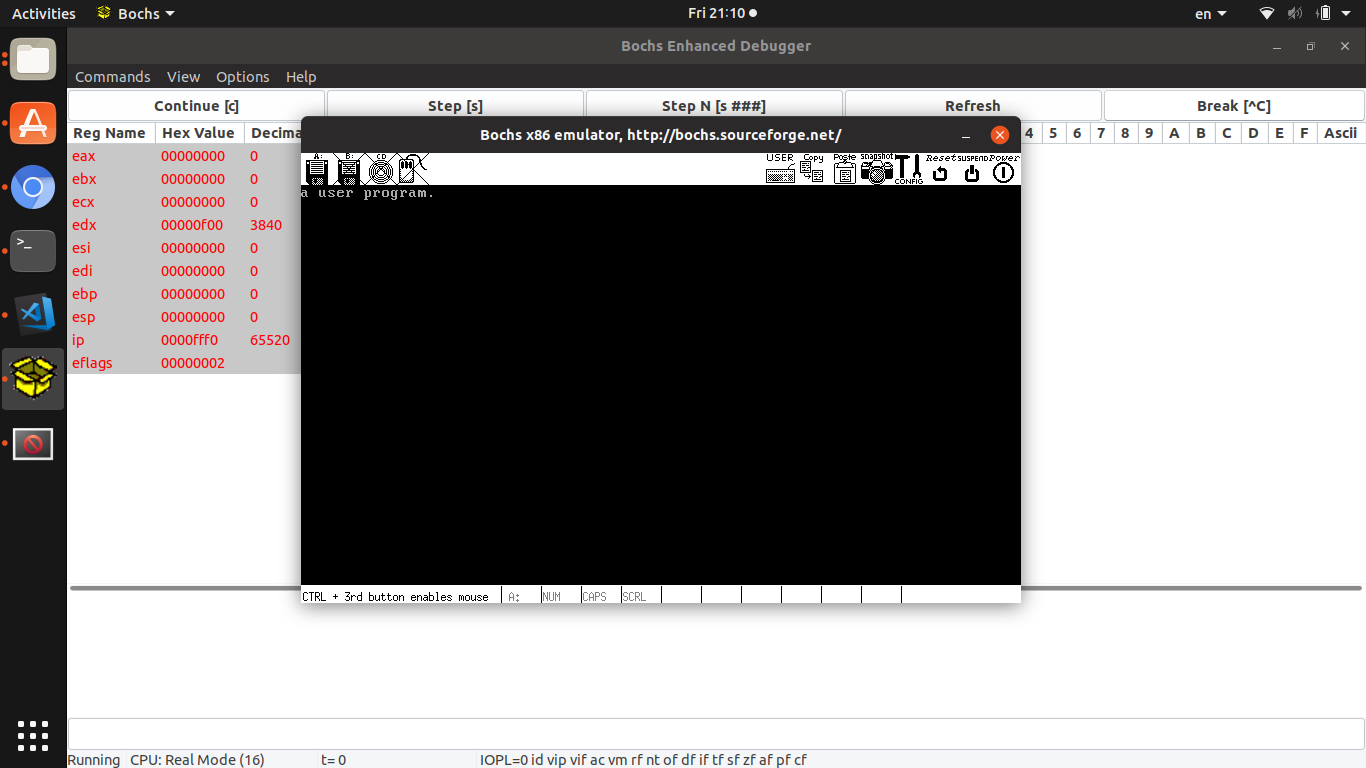
\includegraphics[width=\textwidth]{imgs/Screenshot_from_2019-03-29_21-10-31.png}
    \bottomcaption{\xiaowuhao{Shot3}}
  \end{figure}
  \begin{figure}[!htbp]
    \centering
    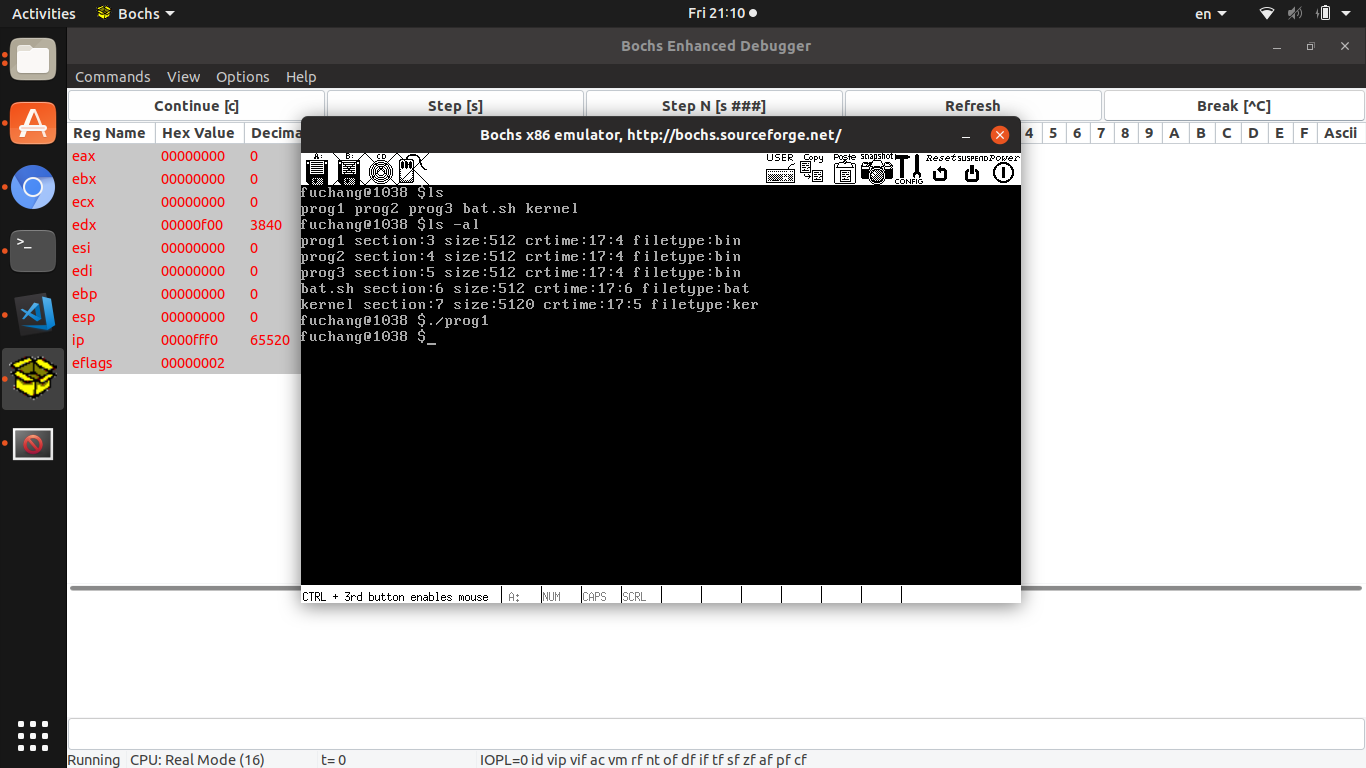
\includegraphics[width=\textwidth]{imgs/Screenshot_from_2019-03-29_21-10-37.png}
    \bottomcaption{\xiaowuhao{Shot3}}
  \end{figure}
  \begin{figure}[!htbp]
    \centering
    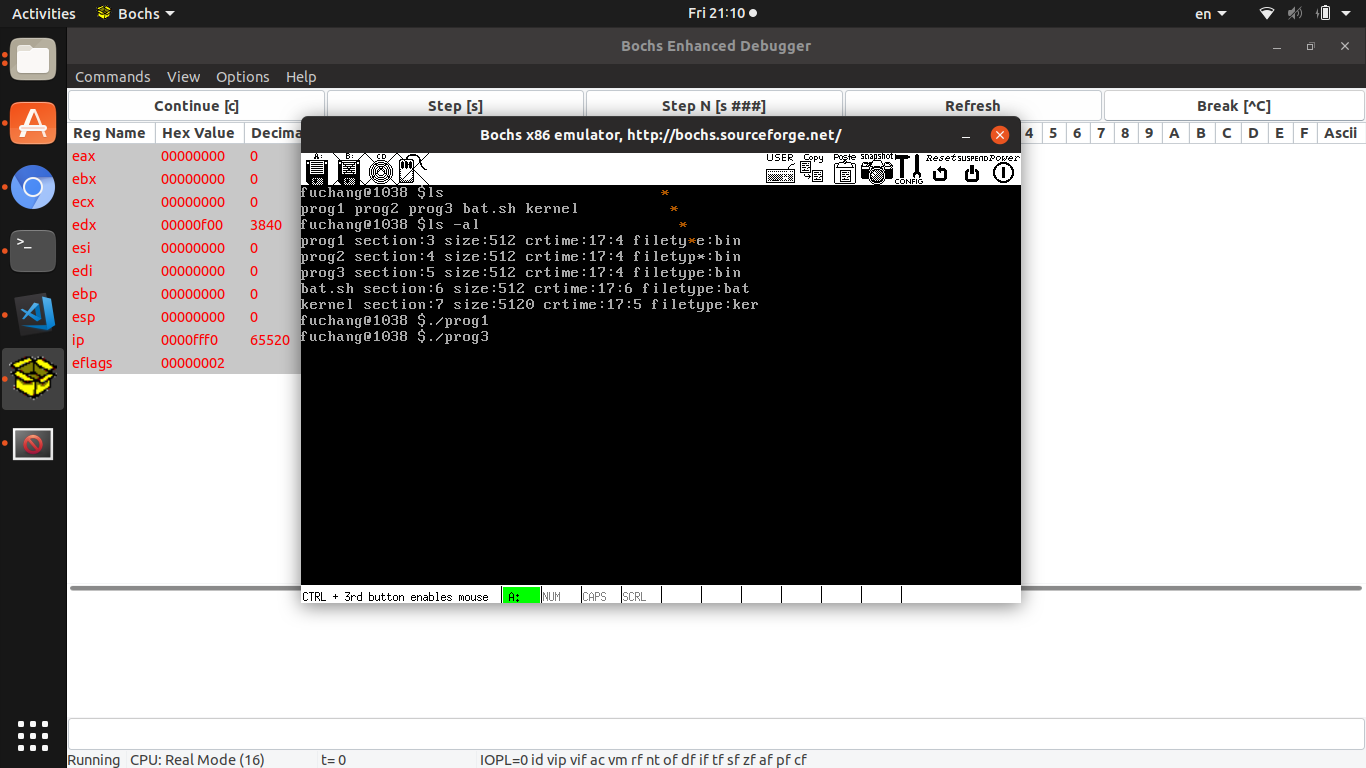
\includegraphics[width=\textwidth]{imgs/Screenshot_from_2019-03-29_21-10-48.png}
    \bottomcaption{\xiaowuhao{Shot3}}
  \end{figure}
  \begin{figure}[!htbp]
    \centering
    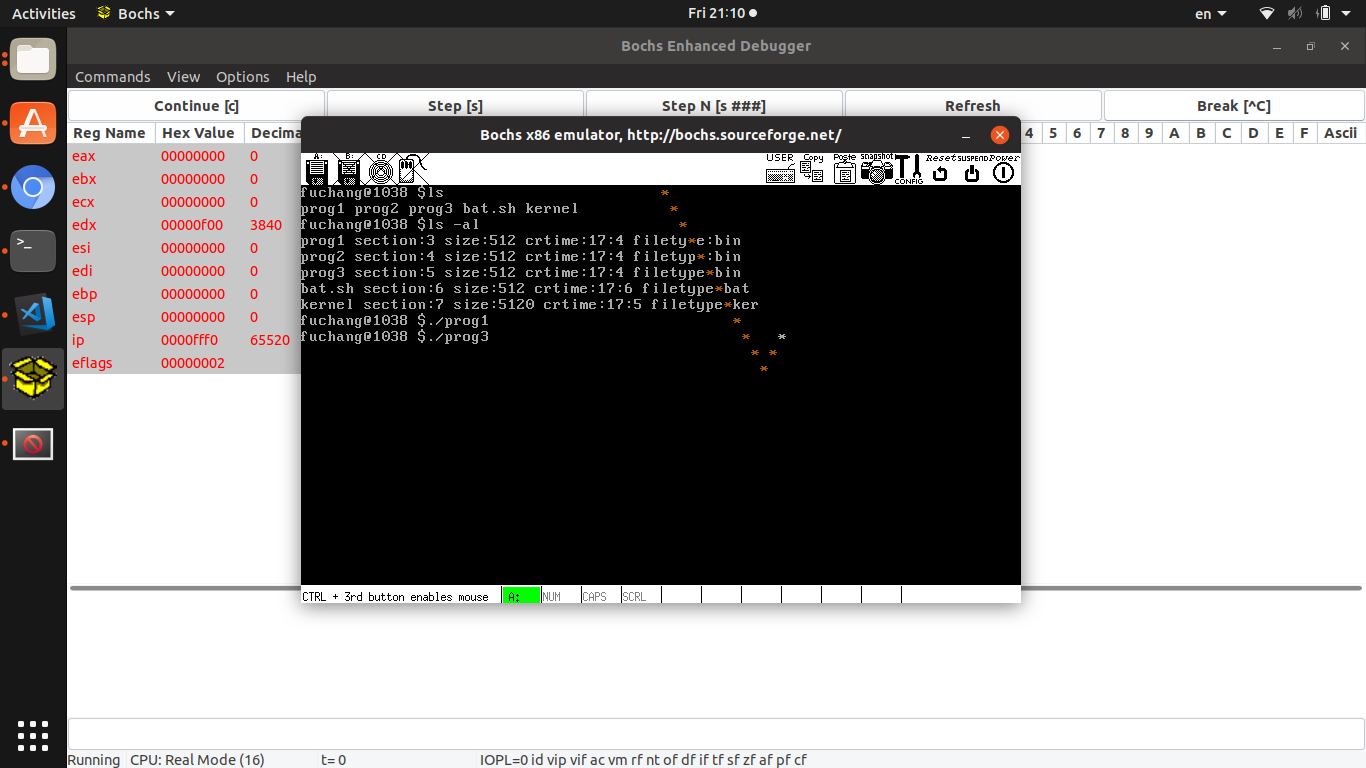
\includegraphics[width=\textwidth]{imgs/Screenshot_from_2019-03-29_21-10-48_-_1.png}
    \bottomcaption{\xiaowuhao{Shot3}}
  \end{figure}
  \begin{figure}[!htbp]
    \centering
    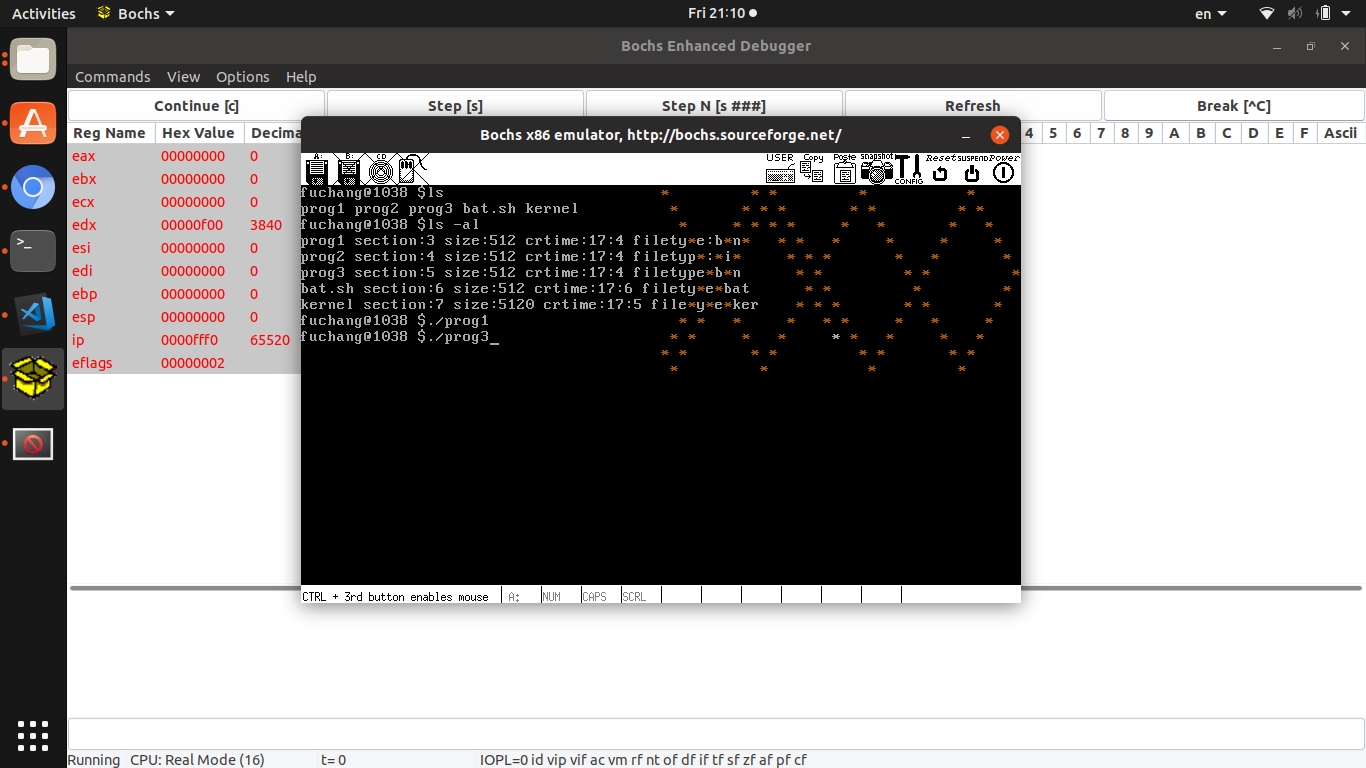
\includegraphics[width=\textwidth]{imgs/Screenshot_from_2019-03-29_21-10-56.png}
    \bottomcaption{\xiaowuhao{Shot3}}
  \end{figure}
  \begin{figure}[!htbp]
    \centering
    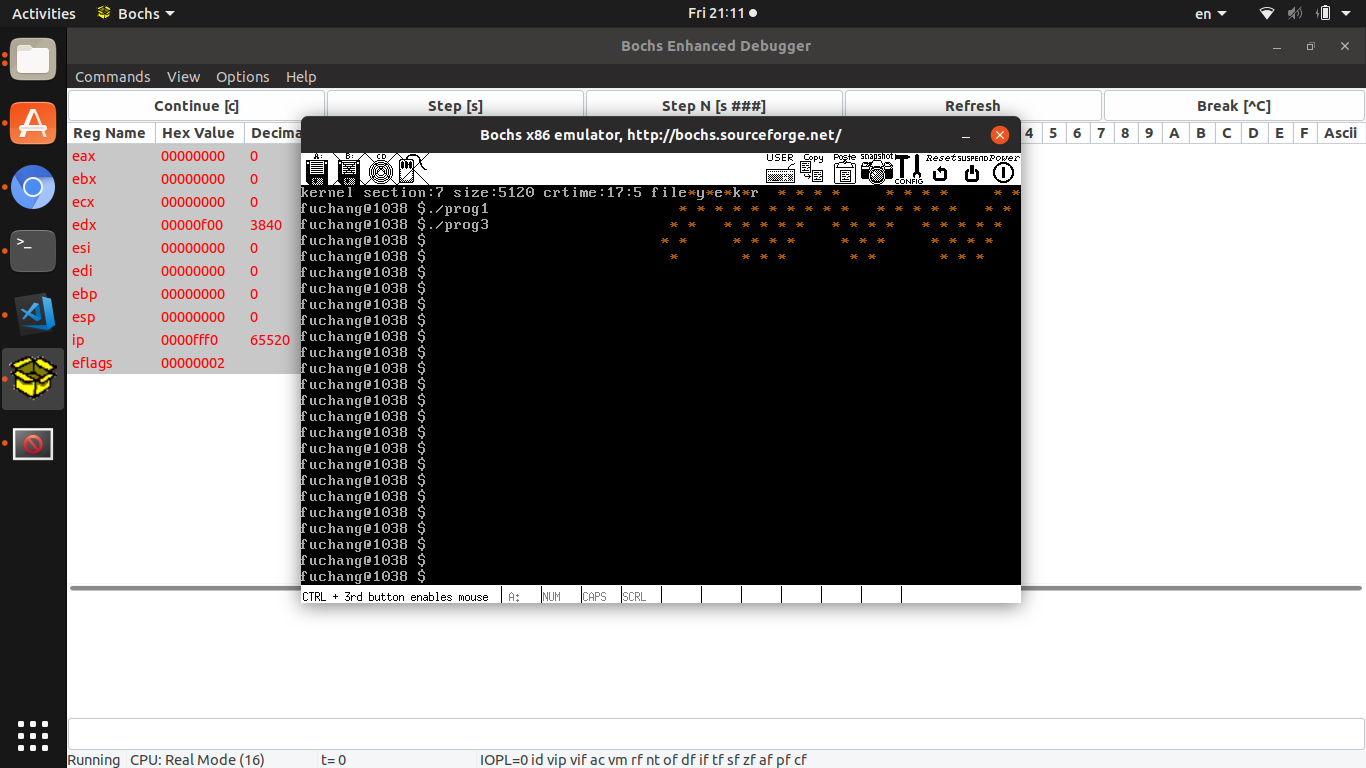
\includegraphics[width=\textwidth]{imgs/Screenshot_from_2019-03-29_21-11-20.png}
    \bottomcaption{\xiaowuhao{Shot3}}
  \end{figure}
  \begin{figure}[!htbp]
    \centering
    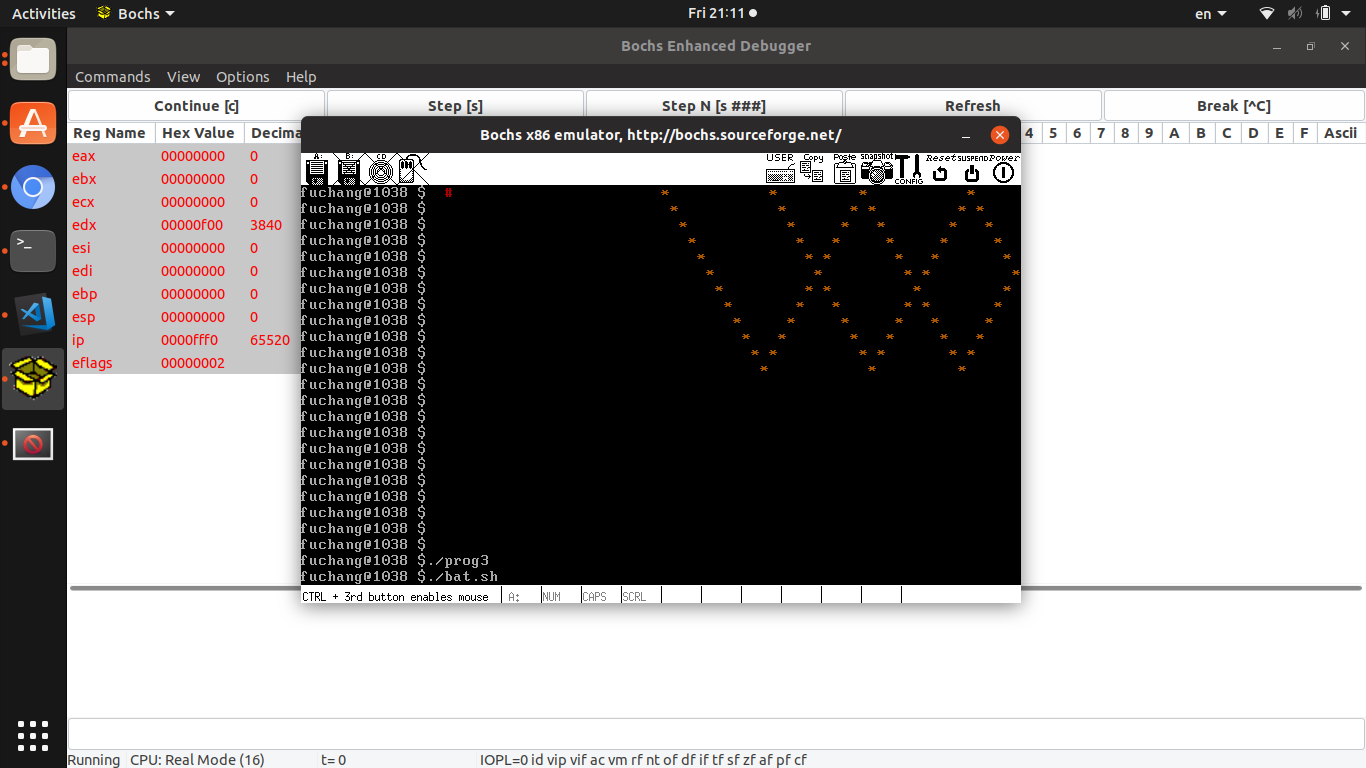
\includegraphics[width=\textwidth]{imgs/Screenshot_from_2019-03-29_21-11-39.png}
    \bottomcaption{\xiaowuhao{Shot3}}
  \end{figure}
  \begin{figure}[!htbp]
    \centering
    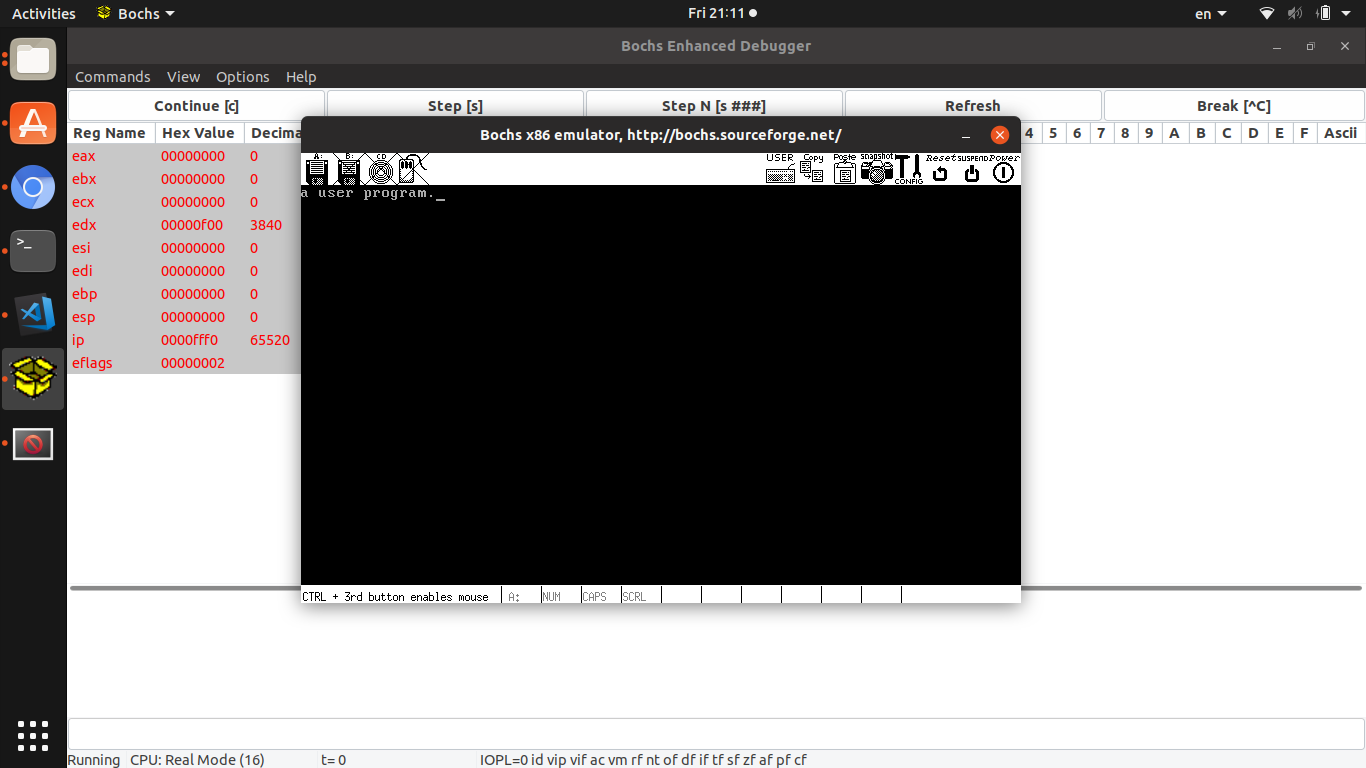
\includegraphics[width=\textwidth]{imgs/Screenshot_from_2019-03-29_21-11-51.png}
    \bottomcaption{\xiaowuhao{Shot3}}
  \end{figure}
(自行填写。每个实验项目的格式范例:
\begin{itemize}
  \item 关键流程分析
  \item 实验结果 \\ 文字描述或者截图(所作的图)。必须有截图,截图数量不少于2幅。
  \item 结果分析 \\ 对每一个结果,必须有相应分析,如解释图表反映的内涵、缘由,是否达到预期目标,是否可改进等等。)
\end{itemize}

\section{总结及心得体会:}

(自行填写。必须写点什么,不能写“无”)

\section{对本实验过程及方法、手段的改进建议:}

(自行填写。必须写点什么,不能写“无”)

(注意:八,九部分能反映出实验的态度、方法和效果,应重点阐述,字数勿少,独立完成,勿参考其他报告,避免雷同)

\vspace{4cm}
\begin{flushright}
\begin{tabular}{lc}
\sihao{\hei{报告评分:}}& \sihao{\hei{X~X~X}}\\
\sihao{\hei{指导教师签字:}}& \sihao{\hei{X~X~X}}\\
\end{tabular}
\end{flushright}

\begin{appendix}

\section{代码示例}

\begin{lstlisting}[caption={一段C代码},captionpos=b]
#include <stdio.h>
int main (int argc, char *argv[]){
  printf("Hello world!");
}
\end{lstlisting}

\section{表格示例}
\begin{table}[!h!tbp]
\caption{一个简单的表格}\label{tab1}
  \centering
  \begin{tabular}{|l|c|c|}
	\hline
	功能          &WEB         &APP         \\ \hline
	注册          &$\surd$     &$\surd$     \\ \hline
	登录          &$\surd$     &$\surd$     \\ \hline
	推送          &$\times$    &$\surd$     \\ \hline
\end{tabular}
\end{table}

\begin{table}[!h!tbp]
\caption{自定义表格}\label{tab2}
  \centering
\begin{tabular*}{0.75\textwidth}{@{\extracolsep{\fill}}lcc}
    \toprule
    功能          &WEB         &APP         \\
    \midrule
    注册          &$\surd$     &$\surd$     \\
    登录          &$\surd$     &$\surd$     \\
    推送          &$\times$    &$\surd$     \\
    \bottomrule
\end{tabular*}
\end{table}


\section{图片示例}

\begin{figure}[!htbp]
\centering

\includegraphics[width=\textwidth]{logo}
\bottomcaption{\xiaowuhao{电子科技大学}}
\end{figure}

\begin{algorithm}
\caption{某个算法}
\begin{algorithmic}[1]  %每行显示行号
\Require 某个输入
\Ensure 某个输出
\Function {函数名} {参数列表}
    \State 某个变量  $\gets$ 某个变量
\EndFunction
\end{algorithmic}
\end{algorithm}

\section{字体示例}
\hei{黑体}
\hwxk{华文行楷}

\end{appendix}

\end{document}
